\chapter{Methodology}
\label{ch:methods}

This chapter outlines the complete methodological workflow — from preprocessing and modeling, to evaluation. Table~\ref{tab:method_summary} provides a cross-dataset overview.

\begin{table}[H]
    \centering
    \caption{Dataset-wise methodology summary}
    \label{tab:method_summary}
    \begin{tabular}{|c|c|c|c|}
        \hline
        \textbf{Dataset} & \textbf{Task Type} & \textbf{Model(s)} & \textbf{Evaluation} \\
        \hline
        Raisin & Classification & KNN, Naïve Bayes & Accuracy, Confusion Matrix \\
        HTRU2 & Classification & KNN, Naïve Bayes & Accuracy, Confusion Matrix \\
        Parking & Clustering & K-Means & Elbow Method, Cluster Plot \\
        \hline
    \end{tabular}
\end{table}

\section{Preprocessing}

All datasets were cleaned, checked for nulls, and scaled. Labels were encoded in classification datasets. Feature selection and subset testing were implemented in loops.

\section{Classification Models}

\subsection{KNN: Distance-Based Learning}
\label{sec:method_knn}

KNN predicts class based on proximity to neighbors. Below is the core implementation:

\begin{lstlisting}[language=Python, caption={KNN implementation snippet}, label=list:knn_code]
model = KNeighborsClassifier(n_neighbors=3)
model.fit(X_train, y_train)
y_pred = model.predict(X_test)
\end{lstlisting}

The conceptual diagram of KNN (Figure~\ref{fig:knn_diagram}) was adapted from Machine Learning Geek \cite{knn_diagram}.

\begin{figure}[H]
    \centering
    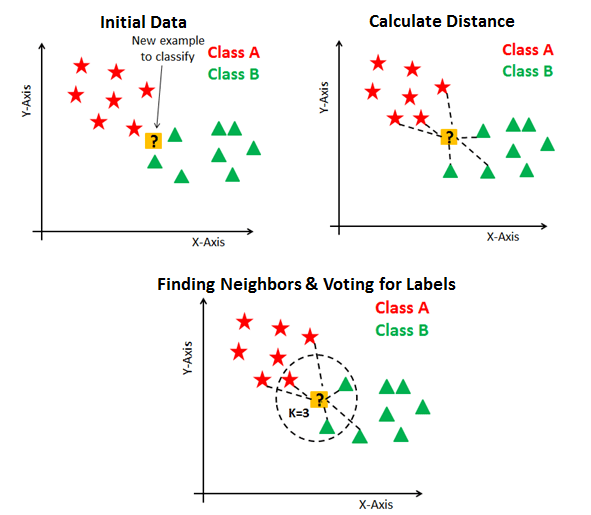
\includegraphics[width=0.5\textwidth]{figures/knn_illustration.png}
    \caption{KNN classification: class based on proximity}
    \label{fig:knn_diagram}
\end{figure}

\subsection{Naïve Bayes: Probabilistic Model}
\label{sec:method_nb}

Naïve Bayes assumes feature independence. This is well-suited for numeric continuous data. The Naïve Bayes visual (Figure~\ref{fig:nb_diagram}) is based on an illustration by Valigi \cite{naive_bayes_diagram}.

\begin{lstlisting}[language=Python, caption={Naïve Bayes model snippet}, label=list:nb_code]
model = GaussianNB()
model.fit(X_train, y_train)
y_pred = model.predict(X_test)
\end{lstlisting}

\begin{figure}[H]
    \centering
    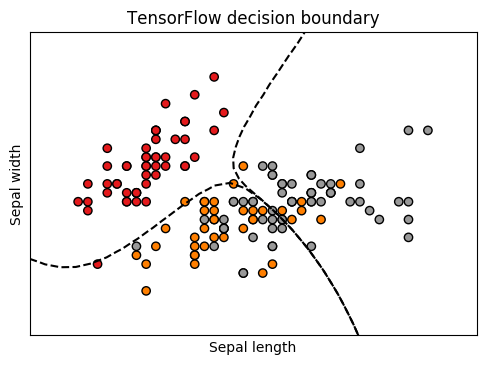
\includegraphics[width=0.5\textwidth]{figures/naive_bayes_concept.png}
    \caption{Naïve Bayes classification using probability distributions}
    \label{fig:nb_diagram}
\end{figure}

\section{Clustering with K-Means}

K-Means partitions data into $K$ clusters by minimizing within-cluster variance.

\begin{lstlisting}[language=Python, caption={Elbow Method for K selection}, label=list:kmeans_code]
inertia = []
for k in range(1, 11):
    kmeans = KMeans(n_clusters=k).fit(X_scaled)
    inertia.append(kmeans.inertia_)
\end{lstlisting}

\begin{figure}[H]
    \centering
    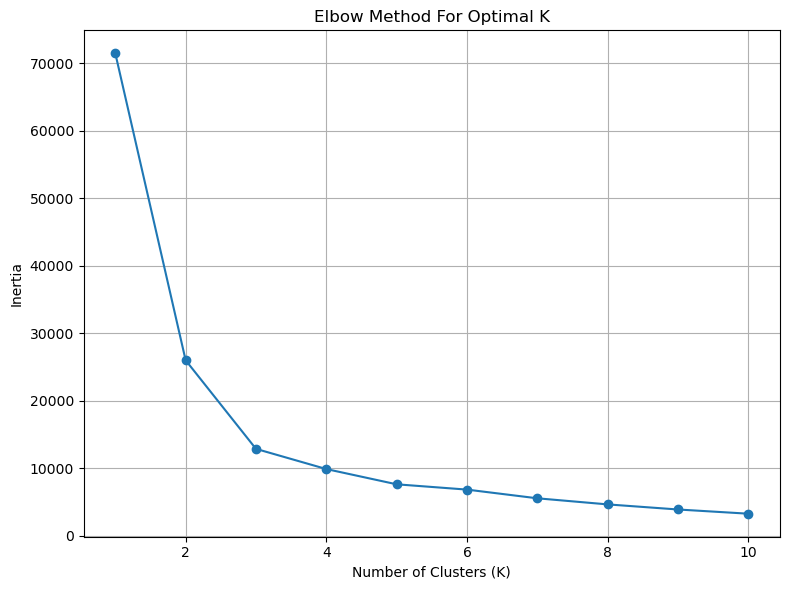
\includegraphics[width=0.6\textwidth]{figures/kmeans_elbow.png}
    \caption{Elbow curve to select optimal K in clustering}
    \label{fig:elbow_curve}
\end{figure}

\section{Incremental Feature Testing}

Both classification models were tested with increasing feature subsets. Table~\ref{tab:feature_growth} shows the progression in Raisin dataset.

\begin{table}[H]
    \centering
    \caption{Feature expansion strategy for Raisin}
    \label{tab:feature_growth}
    \begin{tabular}{|c|l|}
        \hline
        \# Features & Features Used \\
        \hline
        2 & Area, MajorAxisLength \\
        3 & + MinorAxisLength \\
        4 & + Eccentricity \\
        5 & + ConvexArea \\
        6 & + Extent \\
        7 & + Perimeter \\
        \hline
    \end{tabular}
\end{table}

\section{Summary}

This chapter outlined the experimental pipeline used throughout the project. Modular, repeatable, and visual by design, this methodology serves as the foundation for the detailed results in Chapter~\ref{ch:experiments}. All models were implemented using the \texttt{scikit-learn} library in Python \cite{sklearn}.